\documentclass[11pt,a4paper]{article}
\usepackage[margin=17mm]{geometry}
\usepackage[T1]{fontenc}
\usepackage{lmodern}
\usepackage{graphicx,xcolor,booktabs,hyperref}
\definecolor{ink}{HTML}{243548}
\definecolor{teal}{HTML}{237E8A}
\definecolor{muted}{HTML}{5E6D7D}
\hypersetup{colorlinks=true,urlcolor=teal,linkcolor=teal}
\pagestyle{empty}
\setlength{\parindent}{0pt}
\setlength{\parskip}{5pt}
\graphicspath{{../../figures/ManiGuard/phase3-recovery/}}
\begin{document}
\color{ink}
{\small\sffamily\color{teal} SAFETY DIAL / SUPERVISOR CHECK-IN / 19 OCTOBER 2026}\par
{\LARGE\bfseries A working repair, with the physical benefit still to test}\par
{\small Sachin Mohan, 2699183 \hfill Supervisor: Geraud Nangue Tasse}\par
\vspace{1mm}\hrule\vspace{2mm}

\textbf{Research question.} Can evolutionary search find a compact execution
controller that improves safe completion around a frozen manipulation policy,
under matched interaction budgets?

\textbf{Completed today.} Implemented and tested a uniform cap that scales the
whole seven-joint target-error vector, preserving its direction. Ran a frozen
saved-trace diagnostic on \textbf{18,657 commands from 24 historical episodes}.
Prepared a paper with three algorithms, explicit controller equations and audited
outcomes, plus labelled historical demonstration videos.

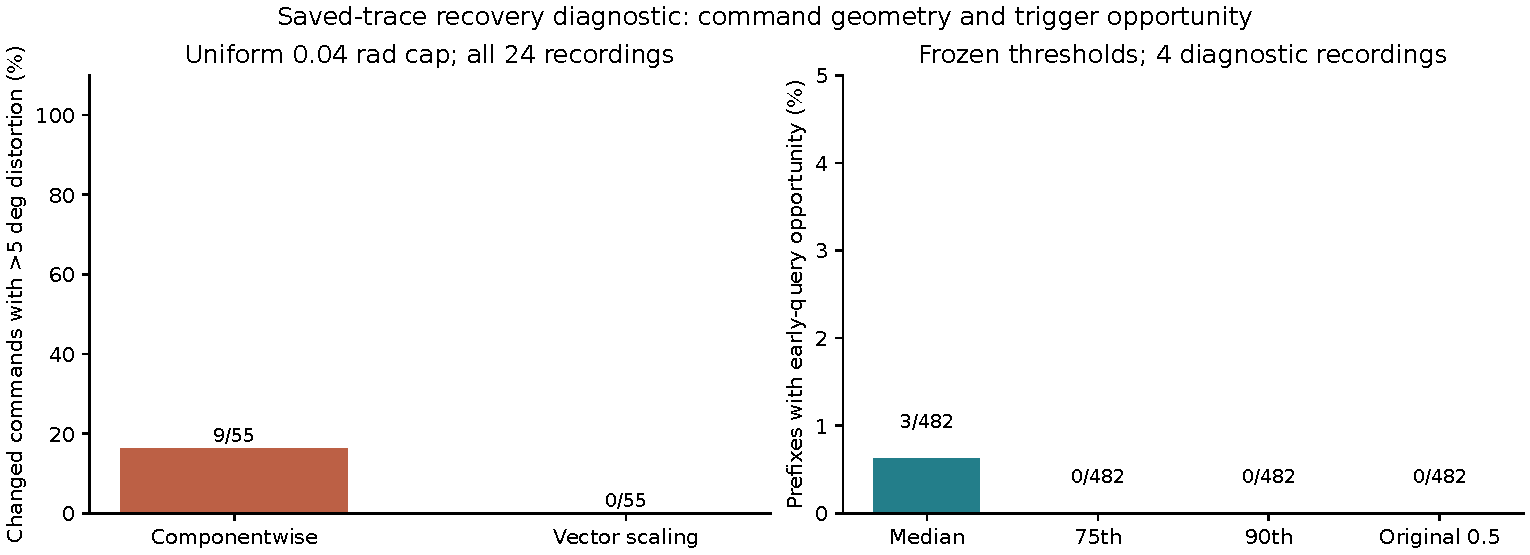
\includegraphics[width=\linewidth]{diagnostic.pdf}

\begin{minipage}[t]{.485\linewidth}
\textbf{Concrete new result}\par
At a .04 rad cap, componentwise clipping rotates joint-error direction by more
than $5^\circ$ on \textbf{9/55} modified commands. Vector scaling has
\textbf{0/55}, with maximum numerical deviation $0.00019^\circ$.
This verifies a command-geometry property; it does not measure physical safety.
\end{minipage}\hfill
\begin{minipage}[t]{.485\linewidth}
\textbf{What limits the timing mechanism}\par
The median threshold .089753 admits \textbf{3/482} early-query opportunities,
all on one of two diagnostic tasks. Calibration has only five positive eligible
values. These are correlated recorded-prefix opportunities, not executed queries
or a new safety result.
\end{minipage}

\vspace{2mm}
\textbf{Physical evidence retained, including the adverse result}\par
\begin{center}
\footnotesize
\begin{tabular}{lrrl}
\toprule
Comparison & Safe completion & Violating episodes & Interpretation \\
\midrule
Part 1 identity & 5/8 & 0/8 & Original policy reference \\
Part 1 full evolved dial & 4/8 & 2/8 & Training lead did not transfer \\
Part 2 identity / cap-8 / adaptive & 3/4 each & 1/4 each & Adaptive rule never refreshed early \\
Part 2 cap-4 & 2/4 & 1/4 & More queries did not improve this pilot \\
\bottomrule
\end{tabular}
\end{center}
\vspace{-2mm}
\textbf{Next decision.} Run the recovery plan's eight-episode mechanism screen:
two preselected development tasks crossed with identity, componentwise cap/8,
vector cap/8 and vector cap with active refresh. Freeze the cap, threshold and
cases first. A later contribution claim needs matched random search and ordinary
learning, independent optimizer seeds and reserved evaluation tasks.

\textbf{Meeting materials.} Open \href{supervisor-draft.pdf}{the paper draft} for
methods and full interpretation. The video package contains a selected full-dial
success, an all-settings-safe case and an adverse case, retaining both cameras and
native timing. Examples were chosen after outcomes; the pooled result remains above.

{\footnotesize\color{muted}
Scope: this machine has no installed ManiGuard simulation/policy stack; the user
selected saved-trace work. Today's diagnostic adds zero simulator controls, physics
steps, VLA queries, encoder calls or trained models. The native monitor labels
violations and does not filter actions. No new physical improvement or optimizer
superiority is claimed.}
\end{document}
